\subsection{Caso d'uso UC7: Creazione nuova infografica}
\begin{figure}[h] 
	\centering 
	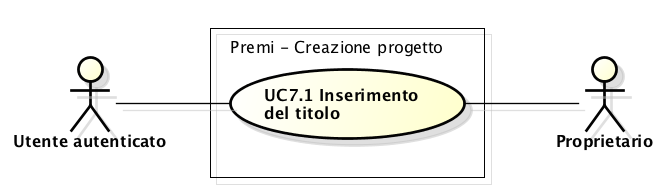
\includegraphics[scale=0.45] {img/UC7.png} 
	\caption{UC7 - Creazione nuova infografica} 
\end{figure}

\begin{itemize}
	\item \textbf{Attori:} Utente;
	\item \textbf{Scopo e descrizione:} L'utente sta creando una nuova infografica. Per completare l'operazione deve scegliere un template e inserire almeno un elemento grafico o testuale. Potrà anche inserire: caselle di testo, immagini, dati \gls{real time}, tabelle, grafici. Potrà scegliere un template predefinito da utilizzare;
	\item \textbf{Precondizione:} Il sistema mostra la schermata di creazione di un'infografica e l'utente vuole scegliere il template;
	\item \textbf{Flusso degli eventi:}
	\begin{enumerate}
		\item L'utente sceglie il template [UC7.1];
		\item L'utente cambia il template [UC7.7];
		\item L'utente può inserire un'immagine o più [UC7.2];
		\item L'utente carica un file per inserire l'immagine [UC7.8];
		\item L'utente può inserire una casella di testo o più [UC7.3];
		\item L'utente sceglie la formattazione del testo [UC7.9];
		\item L'utente può inserire dei dati \gls{real time} [UC7.4];
		\item L'utente può inserire una tabella o più [UC7.5];
		\item L'utente personalizza la tabella [UC7.10];
		\item L'utente può inserire uno o più grafici [UC7.6];
		\item L'utente personalizza il grafico [UC7.11];		
	\end{enumerate}
	\item \textbf{Postcondizione:} Il sistema mostra le operazioni effettuate dall'utente.
\end{itemize}


\subsection{Caso d'uso UC7.1: Scegliere template}
\begin{itemize}
	\item \textbf{Attori:} Utente;
	\item \textbf{Scopo e descrizione:} L'utente sceglie il template con cui creare l'infografica;
	\item \textbf{Precondizione:} Il sistema è in attesa che l'utente scelga il template;
	\item \textbf{Postcondizione:} Il sistema carica il template selezionato.
\end{itemize}


\subsection{Caso d'uso UC7.2: Inserire immagine}
\begin{itemize}
\item \textbf{Attori:} Utente;
\item \textbf{Scopo e descrizione:} L'utente deve inserire l'immagine da mettere nell'infografica;
\item \textbf{Precondizione:} Il sistema è in attesa che l'utente selezioni l'immagine;
\item \textbf{Postcondizione:} Il sistema ha caricato l'immagine selezionata dall'utente.
\end{itemize}


\subsection{Caso d'uso UC7.3: Inserire casella di testo}
\begin{itemize}
\item \textbf{Attori:} Utente;
\item \textbf{Scopo e descrizione:} L'utente deve inserire una casella di testo nella slide;
\item \textbf{Precondizione:} Il sistema è in attesa che l'utente crei una casella di testo;
\item \textbf{Postcondizione:} Il sistema ha creato la casella di testo.
\end{itemize}


\subsection{Caso d'uso UC7.4: Inserire dati real time}
\begin{itemize}
	\item \textbf{Attori:} Utente;
	\item \textbf{Scopo e descrizione:} L'utente deve inserire dei dati \gls{real time};
	\item \textbf{Precondizione:} Il sistema è in attesa che l'utente inserisca i dati \gls{real time};
	\item \textbf{Postcondizione:} Il sistema ha inserito i dati \gls{real time}.
\end{itemize}


\subsection{Caso d'uso UC7.5: Inserire tabella}
\begin{figure}[h] 
	\centering 
	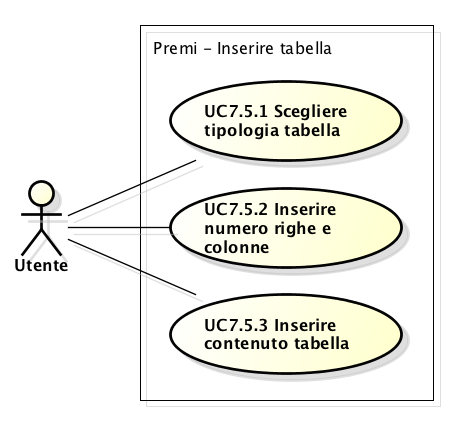
\includegraphics[scale=0.45] {img/UC7.5.png} 
	\caption{UC7.5 - Inserire tabella} 
\end{figure}

\begin{itemize}
	\item \textbf{Attori:} Utente;
	\item \textbf{Scopo e descrizione:} L'utente deve inserire una tabella. Seleziona il tipo di tabella, il numero di righe e di colonne e inserisce i dati;
	\item \textbf{Precondizione:} Il sistema è in attesa che l'utente crei una tabella;
	\item \textbf{Flusso di eventi:}
	\begin{enumerate}
		\item L'utente sceglie la tipologia di tabella da inserire [UC7.5.1];
		\item L'utente inserisce il numero di righe e di colonne [UC7.5.2];
		\item L'utente inserisce i dati all'interno della tabella [UC7.5.3];
	\end{enumerate}
	\item \textbf{Postcondizione:} Il sistema ha creato la tabella.
\end{itemize}

\subsection{Caso d'uso UC7.5.1: Scegliere tipologia tabella}
\begin{itemize}
	\item \textbf{Attori:} Utente;
	\item \textbf{Scopo e descrizione:} L'utente può scegliere il tipo di tabella da inserire;
	\item \textbf{Precondizione:} Il sistema è in attesa che l'utente selezioni il tipo di tabella;
	\item \textbf{Postcondizione:} Il sistema registra la scelta dell'utente.
\end{itemize}

\subsection{Caso d'uso UC7.5.2: Inserire numero di righe e colonne}
\begin{itemize}
	\item \textbf{Attori:} Utente;
	\item \textbf{Scopo e descrizione:} L'utente deve inserire il numero di righe e di colonne per la tabella da inserire;
	\item \textbf{Precondizione:} Il sistema è in attesa che l'utente inserisca il numero di righe e di colonne;
	\item \textbf{Postcondizione:} Il sistema registra l'inserimento dell'utente.
\end{itemize}

\subsection{Caso d'uso UC7.5.3: inserire contenuto tabella}
\begin{itemize}
	\item \textbf{Attori:} Utente;
	\item \textbf{Scopo e descrizione:} L'utente deve inserire il contenuto nelle celle della tabella;
	\item \textbf{Precondizione:} Il sistema è in attesa che l'utente inserisca il contenuto desiderato;
	\item \textbf{Postcondizione:} Il sistema salva il contenuto inserito dall'utente.
\end{itemize}


\subsection{Caso d'uso UC7.6: Inserire grafico}
\begin{figure}[h] 
	\centering 
	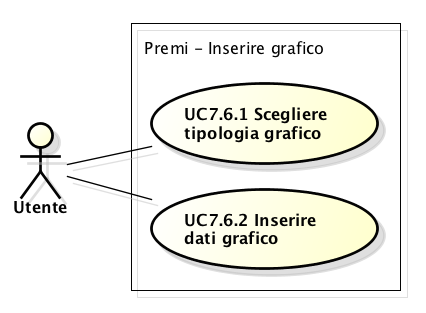
\includegraphics[scale=0.45] {img/UC7.6.png} 
	\caption{UC7.6 - Inserire grafico} 
\end{figure}

\begin{itemize}
	\item \textbf{Attori:} Utente;
	\item \textbf{Scopo e descrizione:} L'utente deve inserire un grafico. Seleziona il tipo di grafico e inserisce i dati;
	\item \textbf{Precondizione:} Il sistema è in attesa che l'utente crei un grafico;
	\item \textbf{Flusso di eventi:}
	\begin{enumerate}
		\item L'utente sceglie la tipologia di grafico da inserire [UC7.6.1];
		\item L'utente inserisce i dati da inserire nel grafico [UC7.6.2];
	\end{enumerate}
	\item \textbf{Postcondizione:} Il sistema ha creato il grafico.
\end{itemize}

\subsection{Caso d'uso UC7.6.1: Scegliere tipologia grafico}
\begin{itemize}
	\item \textbf{Attori:} Utente;
	\item \textbf{Scopo e descrizione:} L'utente può scegliere il tipo di grafico da inserire;
	\item \textbf{Precondizione:} Il sistema è in attesa che l'utente selezioni il tipo di grafico;
	\item \textbf{Postcondizione:} Il sistema registra la scelta dell'utente.
\end{itemize}

\subsection{Caso d'uso UC7.6.2: Inserire dati grafico}
\begin{itemize}
	\item \textbf{Attori:} Utente;
	\item \textbf{Scopo e descrizione:} L'utente deve inserire i dati per il grafico da inserire;
	\item \textbf{Precondizione:} Il sistema è in attesa che l'utente inserisca ii dati;
	\item \textbf{Postcondizione:} Il sistema salva i dati inseriti.
\end{itemize}


\subsection{Caso d'uso UC7.7: Cambiare template}
\begin{itemize}
	\item \textbf{Attori:} Utente;
	\item \textbf{Scopo e descrizione:} L'utente può cambiare template dell'infografica;
	\item \textbf{Precondizione:} Il sistema è in attesa che l'utente selezioni il template;
	\item \textbf{Postcondizione:} Il sistema ha cambiato il template con quello scelto dall'utente.
\end{itemize}


\subsection{Caso d'uso UC7.8: Caricare file}
\begin{figure}[h] 
	\centering 
	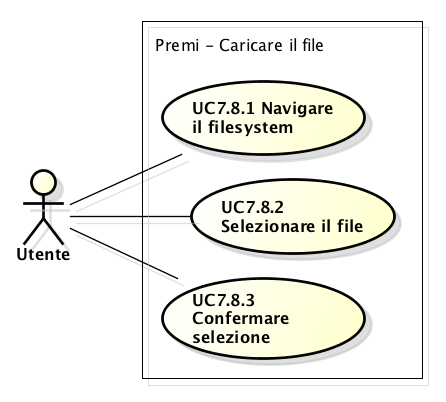
\includegraphics[scale=0.45] {img/UC7.8.png} 
	\caption{UC7.8 - Caricare file} 
\end{figure}

\begin{itemize}
	\item \textbf{Attori:} Utente;
	\item \textbf{Scopo e descrizione:} L'utente deve caricare un file. Naviga il \gls{filesystem} cercando il file desiderato, lo seleziona e conferma la selezione caricando il file;
	\item \textbf{Precondizione:} Il sistema è in attesa che l'utente selezioni il file;
	\item \textbf{Flusso degli eventi:}
	\begin{enumerate}
		\item L'utente naviga il \gls{filesystem} alla ricerca del file desiderato [UC7.8.1];
		\item L'utente seleziona il file [UC7.8.2];
		\item L'utente conferma il file selezionato [UC7.8.3].
	\end{enumerate}
	\item \textbf{Postcondizione:} Il sistema ha caricato il file selezionato dall'utente e lo ha inserito nella slide.
\end{itemize}

\subsection{Caso d'uso UC7.8.1: Navigare il filesystem}
\begin{itemize}
	\item \textbf{Attori:} Utente;
	\item \textbf{Scopo e descrizione:} L'utente può navigare il \gls{filesystem} per selezionare la cartella dentro la quale è contenuto il file desiderato;
	\item \textbf{Precondizione:} Il sistema è in attesa che l'utente selezioni una cartella;
	\item \textbf{Postcondizione:} Il sistema ha aggiornato la cartella corrente con quella scelta dall'utente.
\end{itemize}

\subsection{Caso d'uso UC7.8.2: Selezionare il file}
\begin{itemize}
	\item \textbf{Attori:} Utente;
	\item \textbf{Scopo e descrizione:} L'utente deve selezionare il file che intende caricare;
	\item \textbf{Precondizione:} Il sistema mostra i file contenuti nella cartella precedentemente selezionata;
	\item \textbf{Postcondizione:} Il sistema evidenzia il file scelto dall'utente.
\end{itemize}

\subsection{Caso d'uso UC7.8.3: Confermare selezione}
\begin{itemize}
	\item \textbf{Attori:} Utente;
	\item \textbf{Scopo e descrizione:} L'utente conferma che il file selezionato in precedenza è quello corretto;
	\item \textbf{Precondizione:} Il sistema ha selezionato il file indicato dall'utente;
	\item \textbf{Postcondizione:} Il sistema ha caricato il file scelto precedentemente dall'utente.
\end{itemize}


\subsection{Caso d'uso UC7.9: Scegliere formattazione del testo}
\begin{figure}[h] 
	\centering 
	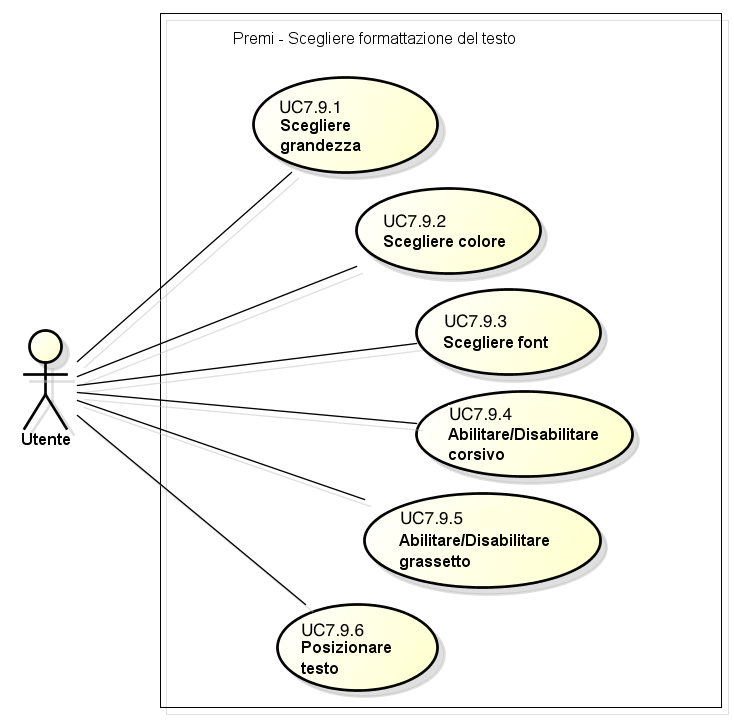
\includegraphics[scale=0.45] {img/UC7.9.png} 
	\caption{UC7.9 - Scegliere formattazione del testo} 
\end{figure}

\begin{itemize}
	\item \textbf{Attori:} Utente;
	\item \textbf{Scopo e descrizione:} L'utente può modificare l'aspetto del testo contenuto in una casella di testo. L'utente seleziona il testo e poi sceglie che modifiche effettuare;
	\item \textbf{Precondizione:} Il sistema è in attesa che l'utente selezioni la modifica da apportare al testo e il testo da modificare è selezionato;
	\item \textbf{Flusso degli eventi:}
	\begin{enumerate}
		\item L'utente può cambiare la grandezza del testo [UC7.9.1];
		\item L'utente può cambiare il colore del testo [UC7.9.2];
		\item L'utente può cambiare il \gls{font} del testo [UC7.9.3];
		\item L'utente può abilitare o disabilitare il testo in corsivo [UC7.9.4];
		\item L'utente può abilitare o disabilitare il testo in grassetto [UC7.9.5];
		\item L'utente può spostare il testo in una nuova posizione [UC7.9.6].
	\end{enumerate}
	\item \textbf{Postcondizione:} Il sistema ha apportato le modifiche scelte al testo.
\end{itemize}

\subsection{Caso d'uso UC7.9.1: Scegliere grandezza}
\begin{itemize}
	\item \textbf{Attori:} Utente;
	\item \textbf{Scopo e descrizione:} L'utente può cambiare la grandezza del testo;
	\item \textbf{Precondizione:} Il testo da modificare è selezionato;
	\item \textbf{Postcondizione:} Il testo è stato ingrandito o rimpicciolito secondo la scelta dell'utente.
\end{itemize}

\subsection{Caso d'uso UC7.9.2: Scegliere colore}
\begin{itemize}
	\item \textbf{Attori:} Utente;
	\item \textbf{Scopo e descrizione:} L'utente può cambiare il colore del testo;
	\item \textbf{Precondizione:} Il testo da modificare è selezionato;
	\item \textbf{Postcondizione:} Il testo è stato colorato secondo la scelta dell'utente.
\end{itemize}

\subsection{Caso d'uso UC7.9.3: Scegliere font}
\begin{itemize}
	\item \textbf{Attori:} Utente;
	\item \textbf{Scopo e descrizione:} L'utente può cambiare il \gls{font} del testo;
	\item \textbf{Precondizione:} Il testo da modificare è selezionato;
	\item \textbf{Postcondizione:} Il testo ha cambiato \gls{font} secondo la scelta dell'utente.
\end{itemize}

\subsection{Caso d'uso UC7.9.4: Abilitare/Disabilitare corsivo}
\begin{itemize}
	\item \textbf{Attori:} Utente;
	\item \textbf{Scopo e descrizione:} L'utente può abilitare o disabilitare la scrittura in corsivo;
	\item \textbf{Precondizione:} Il testo da modificare è selezionato oppure è stata selezionata la casella di testo nella quale poter scrivere;
	\item \textbf{Postcondizione:} Il testo è stato modificato secondo la scelta dell'utente.
\end{itemize}

\subsection{Caso d'uso UC7.9.5: Abilitare/Disabilitare grassetto}
\begin{itemize}
	\item \textbf{Attori:} Utente;
	\item \textbf{Scopo e descrizione:} L'utente può abilitare o disabilitare la scrittura in grassetto;
	\item \textbf{Precondizione:} Il testo da modificare è selezionato oppure è stata selezionata la casella di testo nella quale poter scrivere;
	\item \textbf{Postcondizione:} Il testo è stato modificato secondo la scelta dell'utente.
\end{itemize}

\subsection{Caso d'uso UC7.9.6: Posizionare testo}
\begin{itemize}
	\item \textbf{Attori:} Utente;
	\item \textbf{Scopo e descrizione:} L'utente può spostare una casella di testo in una nuova posizione;
	\item \textbf{Precondizione:} La casella di testo da spostare è stata selezionata;
	\item \textbf{Postcondizione:} La casella di testo è stata spostata secondo la scelta dell'utente.
\end{itemize}


\subsection{Caso d'uso UC7.10: Personalizzare tabella}
\begin{figure}[h] 
	\centering 
	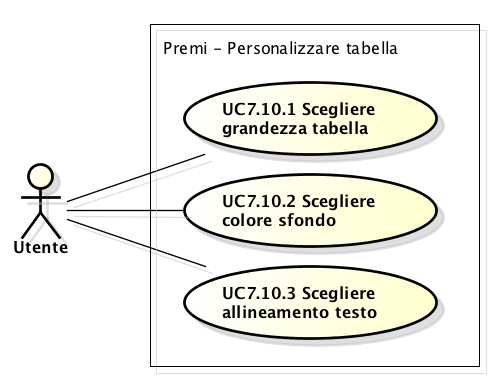
\includegraphics[scale=0.45] {img/UC7.10.png} 
	\caption{UC7.10 - Personalizzare tabella} 
\end{figure}

\begin{itemize}
	\item \textbf{Attori:} Utente;
	\item \textbf{Scopo e descrizione:} L'utente può modificare l'aspetto della tabella e del suo contenuto. L'utente seleziona la tabella o il testo e poi sceglie che modifiche effettuare;
	\item \textbf{Precondizione:} Il sistema è in attesa che l'utente selezioni la modifica da apportare alla tabella e la tabella o il testo da modificare sono selezionati;
	\item \textbf{Flusso degli eventi:}
	\begin{enumerate}
		\item L'utente può cambiare la grandezza della tabella [UC7.10.1];
		\item L'utente può cambiare il colore di sfondo della tabella [UC7.10.2];
		\item L'utente può cambiare l'allineamento del testo [UC7.10.3];
		\item L'utente può cambiare la formattazione del testo [UC7.9];
	\end{enumerate}
	\item \textbf{Postcondizione:} Il sistema ha apportato le modifiche scelte alla tabella.
\end{itemize}

\subsection{Caso d'uso UC7.10.1: Scegliere grandezza tabella}
\begin{itemize}
	\item \textbf{Attori:} Utente;
	\item \textbf{Scopo e descrizione:} L'utente può modificare la grandezza della tabella;
	\item \textbf{Precondizione:} La tabella da modificare è stata selezionata;
	\item \textbf{Postcondizione:} La tabella è stata modificata nelle sue dimensioni secondo la scelta dell'utente.
\end{itemize}

\subsection{Caso d'uso UC7.10.2: Scegliere colore di sfondo tabella}
\begin{itemize}
	\item \textbf{Attori:} Utente;
	\item \textbf{Scopo e descrizione:} L'utente può modificare il colore di sfondo della tabella;
	\item \textbf{Precondizione:} La tabella o le celle da modificare sono state selezionate;
	\item \textbf{Postcondizione:} Lo sfondo della tabella o delle celle è stato modificato secondo la scelta dell'utente.
\end{itemize}

\subsection{Caso d'uso UC7.10.3: Scegliere allineamento del testo}
\begin{itemize}
	\item \textbf{Attori:} Utente;
	\item \textbf{Scopo e descrizione:} L'utente può modificare l'allineamento del testo della tabella;
	\item \textbf{Precondizione:} La tabella o le celle da modificare sono state selezionate;
	\item \textbf{Postcondizione:} L'allineamento del testo della tabella o delle celle è stato modificato secondo la scelta dell'utente.
\end{itemize}


\subsection{Caso d'uso UC7.11: Personalizzare grafico}
\begin{figure}[h] 
	\centering 
	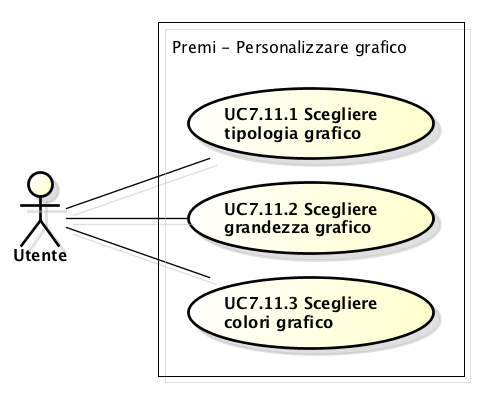
\includegraphics[scale=0.45] {img/UC7.11.png} 
	\caption{UC7.11 - Personalizzare grafico} 
\end{figure}

\begin{itemize}
	\item \textbf{Attori:} Utente;
	\item \textbf{Scopo e descrizione:} L'utente può modificare la tipologia e l'aspetto del grafico o del suo contenuto. L'utente seleziona il grafico e poi sceglie che modifiche effettuare;
	\item \textbf{Precondizione:} Il sistema è in attesa che l'utente selezioni la modifica da apportare al grafico e il grafico da modificare è selezionato;
	\item \textbf{Flusso degli eventi:}
	\begin{enumerate}
		\item L'utente può cambiare la tipologia del grafico [UC7.11.1];
		\item L'utente può cambiare la dimensione del grafico [UC7.11.2]
		\item L'utente può cambiare i colori del grafico [UC7.11.3];
	\end{enumerate}
	\item \textbf{Postcondizione:} Il sistema ha apportato le modifiche scelte al grafico.
\end{itemize}

\subsection{Caso d'uso UC7.11.1: Scegliere tipologia grafico}
\begin{itemize}
	\item \textbf{Attori:} Utente;
	\item \textbf{Scopo e descrizione:} L'utente può modificare la tipologia del grafico;
	\item \textbf{Precondizione:} Il grafico da modificare è stata selezionato;
	\item \textbf{Postcondizione:} La tipologia del grafico è stata modificata secondo la scelta dell'utente.
\end{itemize}

\subsection{Caso d'uso UC7.11.2: Scegliere grandezza grafico}
\begin{itemize}
	\item \textbf{Attori:} Utente;
	\item \textbf{Scopo e descrizione:} L'utente può modificare la grandezza del grafico;
	\item \textbf{Precondizione:} Il grafico da modificare è stata selezionato;
	\item \textbf{Postcondizione:} Il grafico è stata modificato nelle sue dimensioni secondo la scelta dell'utente.
\end{itemize}

\subsection{Caso d'uso UC7.11.3: Scegliere colori grafico}
\begin{itemize}
	\item \textbf{Attori:} Utente;
	\item \textbf{Scopo e descrizione:} L'utente può modificare il set di colori del grafico;
	\item \textbf{Precondizione:} Il grafico da modificare è stata selezionato;
	\item \textbf{Postcondizione:} I colori del grafico sono stati modificati secondo la scelta dell'utente.
\end{itemize}